\documentclass[a4paper, 12pt]{article}
% page
% \usepackage[top=2.54cm,bottom=2.54cm,left=3.18cm,right=3.18cm]{geometry}  % default
\usepackage{graphicx}
\usepackage[top=2.27cm,bottom=1.27cm,left=1.27cm,right=1.27cm]{geometry}
% \usepackage[none]{hyphenat} % remove hyphen

% header and footer
\usepackage{fancyhdr}
\fancypagestyle{plain}{
    \fancyhead[L]{}
    \fancyhead[C]{Computer Vision HW2 Report}
    \fancyhead[R]{Student ID: R11625015\\ Name: 廖致豪}
    % \fancyfoot[L]{}
    % \fancyfoot[C]{}
    % \fancyfoot[R]{}
    \renewcommand{\headrulewidth}{0.5pt}
    \renewcommand{\footrulewidth}{0pt}
    % \setlength{\headheight}{}
    % \addtolength{\topmargin}{}
}
\pagestyle{plain}

% font setting
\usepackage{fontspec}
\usepackage{xeCJK}
    \setCJKmainfont{標楷體}
    % \setCJKmainfont{微軟正黑體}
    \XeTeXlinebreaklocale "zh"
    \XeTeXlinebreakskip = 0pt plus 1pt
    \defaultCJKfontfeatures{AutoFakeBold=true,AutoFakeSlant=true}
    % \newCJKfontfamily\Kai{標楷體}
    \newCJKfontfamily\Hei{微軟正黑體}
    \newCJKfontfamily\NewMing{新細明體}
    \setmainfont{Arial}   % Set English to Arial

% codestyle
\usepackage{listings}
\usepackage{xcolor}
\definecolor{codegreen}{rgb}{0,0.6,0}
\definecolor{codegray}{rgb}{0.5,0.5,0.5}
\definecolor{codepurple}{rgb}{0.58,0,0.82}
\definecolor{backcolour}{rgb}{0.95,0.95,0.92}

\lstdefinestyle{mystyle}{
    backgroundcolor=\color{backcolour},   
    commentstyle=\color{codegreen},
    keywordstyle=\color{magenta},
    numberstyle=\tiny\color{codegray},
    stringstyle=\color{codepurple},
    basicstyle=\ttfamily\footnotesize,
    breakatwhitespace=false,         
    breaklines=true,                 
    captionpos=b,                    
    keepspaces=true,                 
    numbers=left,                    
    numbersep=5pt,                  
    showspaces=false,                
    showstringspaces=false,
    showtabs=false,                  
    tabsize=2
}

\lstset{style=mystyle}

% packages
\usepackage{tabularx, array, slashbox}
\usepackage{makecell}
\usepackage{multirow}
\usepackage{amsmath}
\usepackage{url}
% \usepackage{indentfirst}

% main page
\begin{document}
\section{Part 1. (10\%)}
\subsection{Plot confusion matrix of two settings. (i.e. Bag of sift and tiny image) (5\%)}
\begin{table}[!htb]
    \centering
    \caption{The confusion matrix and the accuracy of bag of sift and tiny image}
    \begin{tabular}{|c|c|}
        \hline
        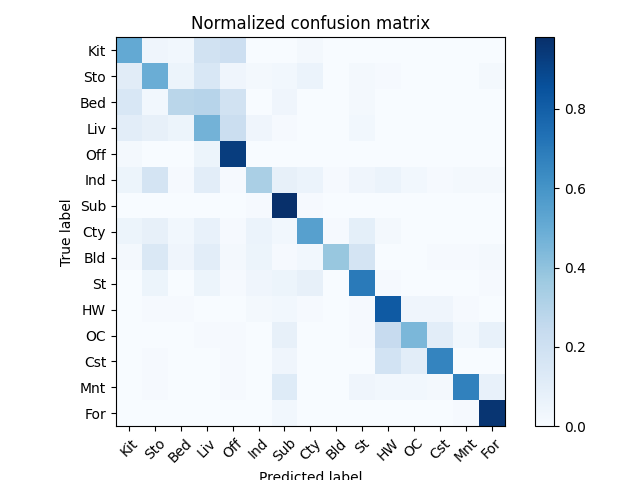
\includegraphics[scale=0.5]{p1/bag_of_sift.png} & 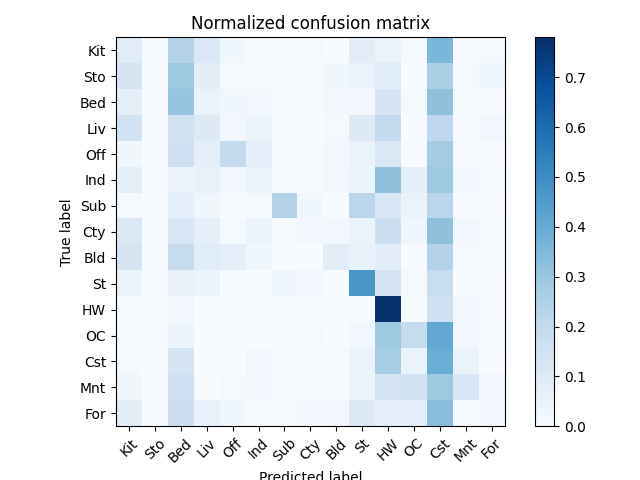
\includegraphics[scale=0.5]{p1/tiny_image.png} \\
        \hline
        bag\_of\_sift = 0.612                           & tiny\_image = 0.2033                           \\
        \hline
    \end{tabular}
\end{table}

\subsection{Compare the results/accuracy of both settings and explain the result. (5\%)}
In the course of model training, there's a multitude of parameters ripe for fine-tuning to maximize performance. As a result, models trained with varying parameter setups showcase discrepancies in accuracy and methodological strategies. Presented below are the outcomes observed across different parameter configurations.

\subsubsection{tiny\_image}
Based on the TODO recommendations, I resized the images to 16 * 16, normalized them, flattened them into one-dimensional vectors, and then calculated the accuracy using the k-nearest neighbors (KNN) algorithm. Within kNN, I utilized cdist to compute distances, and subsequently assigned labels to the nearest k neighbors, employing the mode to determine the predicted value. Based on supplementary recommendations, by considering different metrics to evaluate the distances between features, replacing default metric='euclidean' with metric='cityblock', the accuracy has shown a noticeable improvement.

However, despite these optimizations, the model still fails to surpass the baseline (0.2). Upon delving deeper into the code and closer inspection,  I found that during the normalization process, there is a choice between utilizing either the L1 norm or the L2 norm, with the latter being the default in np.linalg.norm() function. As a result, by switching to the L1 norm for normalization, the model successfully exceeded the baseline threshold of 0.2. Furthermore, recognizing the significance of selecting the appropriate value for k in the k-nearest neighbors algorithm, we have conducted experiments using different values of k in search of the optimal solution.

\vspace{2em}

\begin{align*}
    \text{euclidean}\Rightarrow & d(x,y)=\sqrt{(x_1-y_1)^2+(x_2-y_2)^2} \\
    \text{cityblock}\Rightarrow & d(x,y)=|x_1-y_1|+|x_2-y_2|
\end{align*}

\begin{align*}
    \text{1-norm}\Rightarrow & ||A||_S = \sum_{i,j}abs(a_{i,j})                        \\
    \text{2-norm}\Rightarrow & ||A||_F = \left[\sum_{i,j}abs(a_{i,j})^2\right]^{(1/2)}
\end{align*}

\begin{table}[!htb]
    \centering
    \caption{The accuracy of various values of k in the tiny image KNN algorithm}
    \begin{tabular}{|c|c|c|c|c|c|}
        \hline
                        & k=1    & k=2    & k=3    & k=4    & k=5    \\
        \hline
        \text{Accuracy} & 0.2233 & 0.1787 & 0.1887 & 0.2047 & 0.2020 \\
        \hline
                        & k=6    & k=7    & k=8    & k=9    & k=10   \\
        \hline
        \text{Accuracy} & 0.1980 & 0.2000 & 0.2033 & 0.1980 & 0.2020 \\
        \hline
    \end{tabular}
\end{table}

\subsubsection{bag\_of\_sift}
According to the task description, we understand that our initial step involves extracting feature descriptors from images using dsift, followed by clustering these features to generate a vocabulary (vocab.pkl). Since an image may contain numerous features, we can represent the bag of sift by creating histograms that illustrate the distribution of cluster assignments for features and ultimately classify using KNN.

For the sake of consistency, we keep the same metrics used from tiny images to evaluate the distances, which means only the step size of dsift() function and the step size of kmean() function can be tuned for optimizing the model. When choosing dsift() function parameters, prioritizing a higher number of features per image can enhance the amount of information provided. This typically results in increased accuracy, albeit at the expense of longer computation times.

Consequently, I conducted tests with various sizes, ranging from step=[5, 5], step=[3, 3], down to step=[1, 1], with results aligning as anticipated. Additionally, larger cluster sizes (vocab\_size) tend to yield superior performance, hence I retained the default value (400) here. Nonetheless, opting for a cluster size that is too small noticeably impairs the ability to distinguish features effectively. Lastly, the choice of k value was determined through experimentation to achieve optimal results.

\begin{table}[!htb]
    \centering
    \caption{The accuracy of various values of k in bag of sift KNN algorithm}
    \begin{tabular}{|c|c|c|c|c|c|}
        \hline
                 & k=1    & k=2    & k=3    & k=4    & k=5    \\
        \hline
        Accuracy & 0.5933 & 0.5780 & 0.5820 & 0.5920 & 0.5927 \\
        \hline
                 & k=6    & k=7    & k=8    & k=9    & k=10   \\
        \hline
        Accuracy & 0.5947 & 0.6013 & 0.6120 & 0.6033 & 0.5973 \\
        \hline
    \end{tabular}
\end{table}

\begin{table}[!htb]
    \centering
    \caption{The accuracy of various step sizes of dsift function}
    \begin{tabular}{|c|c|c|c|}
        \hline
            & step=[1, 1] & step=[3, 3] & step=[5, 5] \\
        \hline
        k=8 & 0.6120      & 0.5833      & 0.5453      \\
        \hline
    \end{tabular}
\end{table}

\subsubsection{summary}
The confusion matrix reveals that the bag of sift approach exhibits a more symmetric matrix compared to tiny images, with only a handful of errors concentrated in the upper-left quadrant. Conversely, in the case of tiny images, a significant proportion of instances are directly classified into specific classes such as Cst, HW, Bed, and Kit, resulting in an asymmetric matrix. Consequently, this observation suggests that the bag of sift approach demonstrates higher accuracy when compared to tiny images.

\section{Part 2. (25\%)}
\subsection{Report accuracy of both models on the validation set. (2\%)}
\begin{table}[!htb]
    \centering
    \caption{The accuracy and loss of both models on training and validation set}
    \begin{tabular}{|c|c|c|c|c|c|}
        \hline
        model    & Train Acc & Val Acc & Train Loss & Val Loss & Accuracy = \\
        \hline
        mynet    & 0.97840   & 0.88980 & 0.06605    & 0.39247  & 0.8898     \\
        \hline
        resnet18 & 0.98415   & 0.89860 & 0.05136    & 0.40423  & 0.8918     \\
        \hline
    \end{tabular}
\end{table}

\subsection{Print the network architecture \& number of parameters of both models. What is the main difference between ResNet and other CNN architectures? (5\%)}
\subsubsection{network architecture of mynet model}
\begin{lstlisting}[language=sh]
    MyNet(
        (conv): Sequential(
          (0): Conv2d(3, 192, kernel_size=(3, 3), stride=(1, 1), padding=(1, 1))
          (1): BatchNorm2d(192, eps=1e-05, momentum=0.1, affine=True, track_running_stats=True)
          (2): ReLU(inplace=True)
        )
        (inception_3a): Inception(
          (branch1): BasicConv2d(
            (conv): Conv2d(192, 64, kernel_size=(1, 1), stride=(1, 1), bias=False)
            (bn): BatchNorm2d(64, eps=0.001, momentum=0.1, affine=True, track_running_stats=True)
          )
          (branch2): Sequential(
            (0): BasicConv2d(
              (conv): Conv2d(192, 96, kernel_size=(1, 1), stride=(1, 1), bias=False)
              (bn): BatchNorm2d(96, eps=0.001, momentum=0.1, affine=True, track_running_stats=True)
            )
            (1): BasicConv2d(
              (conv): Conv2d(96, 128, kernel_size=(3, 3), stride=(1, 1), padding=(1, 1), bias=False)
              (bn): BatchNorm2d(128, eps=0.001, momentum=0.1, affine=True, track_running_stats=True)
            )
          )
          (branch3): Sequential(
            (0): BasicConv2d(
              (conv): Conv2d(192, 16, kernel_size=(1, 1), stride=(1, 1), bias=False)
              (bn): BatchNorm2d(16, eps=0.001, momentum=0.1, affine=True, track_running_stats=True)
            )
            (1): BasicConv2d(
              (conv): Conv2d(16, 32, kernel_size=(3, 3), stride=(1, 1), padding=(1, 1), bias=False)
              (bn): BatchNorm2d(32, eps=0.001, momentum=0.1, affine=True, track_running_stats=True)
            )
            (2): BasicConv2d(
              (conv): Conv2d(32, 32, kernel_size=(3, 3), stride=(1, 1), padding=(1, 1), bias=False)
              (bn): BatchNorm2d(32, eps=0.001, momentum=0.1, affine=True, track_running_stats=True)
            )
          )
          (branch4): Sequential(
            (0): MaxPool2d(kernel_size=3, stride=1, padding=1, dilation=1, ceil_mode=False)
            (1): BasicConv2d(
              (conv): Conv2d(192, 32, kernel_size=(1, 1), stride=(1, 1), bias=False)
              (bn): BatchNorm2d(32, eps=0.001, momentum=0.1, affine=True, track_running_stats=True)
            )
          )
        )
        (inception_3b): Inception(
          (branch1): BasicConv2d(
            (conv): Conv2d(256, 128, kernel_size=(1, 1), stride=(1, 1), bias=False)
            (bn): BatchNorm2d(128, eps=0.001, momentum=0.1, affine=True, track_running_stats=True)
          )
          (branch2): Sequential(
            (0): BasicConv2d(
              (conv): Conv2d(256, 128, kernel_size=(1, 1), stride=(1, 1), bias=False)
              (bn): BatchNorm2d(128, eps=0.001, momentum=0.1, affine=True, track_running_stats=True)
            )
            (1): BasicConv2d(
              (conv): Conv2d(128, 192, kernel_size=(3, 3), stride=(1, 1), padding=(1, 1), bias=False)
              (bn): BatchNorm2d(192, eps=0.001, momentum=0.1, affine=True, track_running_stats=True)
            )
          )
          (branch3): Sequential(
            (0): BasicConv2d(
              (conv): Conv2d(256, 32, kernel_size=(1, 1), stride=(1, 1), bias=False)
              (bn): BatchNorm2d(32, eps=0.001, momentum=0.1, affine=True, track_running_stats=True)
            )
            (1): BasicConv2d(
              (conv): Conv2d(32, 96, kernel_size=(3, 3), stride=(1, 1), padding=(1, 1), bias=False)
              (bn): BatchNorm2d(96, eps=0.001, momentum=0.1, affine=True, track_running_stats=True)
            )
            (2): BasicConv2d(
              (conv): Conv2d(96, 96, kernel_size=(3, 3), stride=(1, 1), padding=(1, 1), bias=False)
              (bn): BatchNorm2d(96, eps=0.001, momentum=0.1, affine=True, track_running_stats=True)
            )
          )
          (branch4): Sequential(
            (0): MaxPool2d(kernel_size=3, stride=1, padding=1, dilation=1, ceil_mode=False)
            (1): BasicConv2d(
              (conv): Conv2d(256, 64, kernel_size=(1, 1), stride=(1, 1), bias=False)
              (bn): BatchNorm2d(64, eps=0.001, momentum=0.1, affine=True, track_running_stats=True)
            )
          )
        )
        (maxpool_3): MaxPool2d(kernel_size=3, stride=2, padding=1, dilation=1, ceil_mode=False)
        (inception_4a): Inception(
          (branch1): BasicConv2d(
            (conv): Conv2d(480, 192, kernel_size=(1, 1), stride=(1, 1), bias=False)
            (bn): BatchNorm2d(192, eps=0.001, momentum=0.1, affine=True, track_running_stats=True)
          )
          (branch2): Sequential(
            (0): BasicConv2d(
              (conv): Conv2d(480, 96, kernel_size=(1, 1), stride=(1, 1), bias=False)
              (bn): BatchNorm2d(96, eps=0.001, momentum=0.1, affine=True, track_running_stats=True)
            )
            (1): BasicConv2d(
              (conv): Conv2d(96, 208, kernel_size=(3, 3), stride=(1, 1), padding=(1, 1), bias=False)
              (bn): BatchNorm2d(208, eps=0.001, momentum=0.1, affine=True, track_running_stats=True)
            )
          )
          (branch3): Sequential(
            (0): BasicConv2d(
              (conv): Conv2d(480, 16, kernel_size=(1, 1), stride=(1, 1), bias=False)
              (bn): BatchNorm2d(16, eps=0.001, momentum=0.1, affine=True, track_running_stats=True)
            )
            (1): BasicConv2d(
              (conv): Conv2d(16, 48, kernel_size=(3, 3), stride=(1, 1), padding=(1, 1), bias=False)
              (bn): BatchNorm2d(48, eps=0.001, momentum=0.1, affine=True, track_running_stats=True)
            )
            (2): BasicConv2d(
              (conv): Conv2d(48, 48, kernel_size=(3, 3), stride=(1, 1), padding=(1, 1), bias=False)
              (bn): BatchNorm2d(48, eps=0.001, momentum=0.1, affine=True, track_running_stats=True)
            )
          )
          (branch4): Sequential(
            (0): MaxPool2d(kernel_size=3, stride=1, padding=1, dilation=1, ceil_mode=False)
            (1): BasicConv2d(
              (conv): Conv2d(480, 64, kernel_size=(1, 1), stride=(1, 1), bias=False)
              (bn): BatchNorm2d(64, eps=0.001, momentum=0.1, affine=True, track_running_stats=True)
            )
          )
        )
        (inception_4b): Inception(
          (branch1): BasicConv2d(
            (conv): Conv2d(512, 160, kernel_size=(1, 1), stride=(1, 1), bias=False)
            (bn): BatchNorm2d(160, eps=0.001, momentum=0.1, affine=True, track_running_stats=True)
          )
          (branch2): Sequential(
            (0): BasicConv2d(
              (conv): Conv2d(512, 112, kernel_size=(1, 1), stride=(1, 1), bias=False)
              (bn): BatchNorm2d(112, eps=0.001, momentum=0.1, affine=True, track_running_stats=True)
            )
            (1): BasicConv2d(
              (conv): Conv2d(112, 224, kernel_size=(3, 3), stride=(1, 1), padding=(1, 1), bias=False)
              (bn): BatchNorm2d(224, eps=0.001, momentum=0.1, affine=True, track_running_stats=True)
            )
          )
          (branch3): Sequential(
            (0): BasicConv2d(
              (conv): Conv2d(512, 24, kernel_size=(1, 1), stride=(1, 1), bias=False)
              (bn): BatchNorm2d(24, eps=0.001, momentum=0.1, affine=True, track_running_stats=True)
            )
            (1): BasicConv2d(
              (conv): Conv2d(24, 64, kernel_size=(3, 3), stride=(1, 1), padding=(1, 1), bias=False)
              (bn): BatchNorm2d(64, eps=0.001, momentum=0.1, affine=True, track_running_stats=True)
            )
            (2): BasicConv2d(
              (conv): Conv2d(64, 64, kernel_size=(3, 3), stride=(1, 1), padding=(1, 1), bias=False)
              (bn): BatchNorm2d(64, eps=0.001, momentum=0.1, affine=True, track_running_stats=True)
            )
          )
          (branch4): Sequential(
            (0): MaxPool2d(kernel_size=3, stride=1, padding=1, dilation=1, ceil_mode=False)
            (1): BasicConv2d(
              (conv): Conv2d(512, 64, kernel_size=(1, 1), stride=(1, 1), bias=False)
              (bn): BatchNorm2d(64, eps=0.001, momentum=0.1, affine=True, track_running_stats=True)
            )
          )
        )
        (inception_4c): Inception(
          (branch1): BasicConv2d(
            (conv): Conv2d(512, 128, kernel_size=(1, 1), stride=(1, 1), bias=False)
            (bn): BatchNorm2d(128, eps=0.001, momentum=0.1, affine=True, track_running_stats=True)
          )
          (branch2): Sequential(
            (0): BasicConv2d(
              (conv): Conv2d(512, 128, kernel_size=(1, 1), stride=(1, 1), bias=False)
              (bn): BatchNorm2d(128, eps=0.001, momentum=0.1, affine=True, track_running_stats=True)
            )
            (1): BasicConv2d(
              (conv): Conv2d(128, 256, kernel_size=(3, 3), stride=(1, 1), padding=(1, 1), bias=False)
              (bn): BatchNorm2d(256, eps=0.001, momentum=0.1, affine=True, track_running_stats=True)
            )
          )
          (branch3): Sequential(
            (0): BasicConv2d(
              (conv): Conv2d(512, 24, kernel_size=(1, 1), stride=(1, 1), bias=False)
              (bn): BatchNorm2d(24, eps=0.001, momentum=0.1, affine=True, track_running_stats=True)
            )
            (1): BasicConv2d(
              (conv): Conv2d(24, 64, kernel_size=(3, 3), stride=(1, 1), padding=(1, 1), bias=False)
              (bn): BatchNorm2d(64, eps=0.001, momentum=0.1, affine=True, track_running_stats=True)
            )
            (2): BasicConv2d(
              (conv): Conv2d(64, 64, kernel_size=(3, 3), stride=(1, 1), padding=(1, 1), bias=False)
              (bn): BatchNorm2d(64, eps=0.001, momentum=0.1, affine=True, track_running_stats=True)
            )
          )
          (branch4): Sequential(
            (0): MaxPool2d(kernel_size=3, stride=1, padding=1, dilation=1, ceil_mode=False)
            (1): BasicConv2d(
              (conv): Conv2d(512, 64, kernel_size=(1, 1), stride=(1, 1), bias=False)
              (bn): BatchNorm2d(64, eps=0.001, momentum=0.1, affine=True, track_running_stats=True)
            )
          )
        )
        (inception_4d): Inception(
          (branch1): BasicConv2d(
            (conv): Conv2d(512, 112, kernel_size=(1, 1), stride=(1, 1), bias=False)
            (bn): BatchNorm2d(112, eps=0.001, momentum=0.1, affine=True, track_running_stats=True)
          )
          (branch2): Sequential(
            (0): BasicConv2d(
              (conv): Conv2d(512, 144, kernel_size=(1, 1), stride=(1, 1), bias=False)
              (bn): BatchNorm2d(144, eps=0.001, momentum=0.1, affine=True, track_running_stats=True)
            )
            (1): BasicConv2d(
              (conv): Conv2d(144, 288, kernel_size=(3, 3), stride=(1, 1), padding=(1, 1), bias=False)
              (bn): BatchNorm2d(288, eps=0.001, momentum=0.1, affine=True, track_running_stats=True)
            )
          )
          (branch3): Sequential(
            (0): BasicConv2d(
              (conv): Conv2d(512, 32, kernel_size=(1, 1), stride=(1, 1), bias=False)
              (bn): BatchNorm2d(32, eps=0.001, momentum=0.1, affine=True, track_running_stats=True)
            )
            (1): BasicConv2d(
              (conv): Conv2d(32, 64, kernel_size=(3, 3), stride=(1, 1), padding=(1, 1), bias=False)
              (bn): BatchNorm2d(64, eps=0.001, momentum=0.1, affine=True, track_running_stats=True)
            )
            (2): BasicConv2d(
              (conv): Conv2d(64, 64, kernel_size=(3, 3), stride=(1, 1), padding=(1, 1), bias=False)
              (bn): BatchNorm2d(64, eps=0.001, momentum=0.1, affine=True, track_running_stats=True)
            )
          )
          (branch4): Sequential(
            (0): MaxPool2d(kernel_size=3, stride=1, padding=1, dilation=1, ceil_mode=False)
            (1): BasicConv2d(
              (conv): Conv2d(512, 64, kernel_size=(1, 1), stride=(1, 1), bias=False)
              (bn): BatchNorm2d(64, eps=0.001, momentum=0.1, affine=True, track_running_stats=True)
            )
          )
        )
        (inception_4e): Inception(
          (branch1): BasicConv2d(
            (conv): Conv2d(528, 256, kernel_size=(1, 1), stride=(1, 1), bias=False)
            (bn): BatchNorm2d(256, eps=0.001, momentum=0.1, affine=True, track_running_stats=True)
          )
          (branch2): Sequential(
            (0): BasicConv2d(
              (conv): Conv2d(528, 160, kernel_size=(1, 1), stride=(1, 1), bias=False)
              (bn): BatchNorm2d(160, eps=0.001, momentum=0.1, affine=True, track_running_stats=True)
            )
            (1): BasicConv2d(
              (conv): Conv2d(160, 320, kernel_size=(3, 3), stride=(1, 1), padding=(1, 1), bias=False)
              (bn): BatchNorm2d(320, eps=0.001, momentum=0.1, affine=True, track_running_stats=True)
            )
          )
          (branch3): Sequential(
            (0): BasicConv2d(
              (conv): Conv2d(528, 32, kernel_size=(1, 1), stride=(1, 1), bias=False)
              (bn): BatchNorm2d(32, eps=0.001, momentum=0.1, affine=True, track_running_stats=True)
            )
            (1): BasicConv2d(
              (conv): Conv2d(32, 128, kernel_size=(3, 3), stride=(1, 1), padding=(1, 1), bias=False)
              (bn): BatchNorm2d(128, eps=0.001, momentum=0.1, affine=True, track_running_stats=True)
            )
            (2): BasicConv2d(
              (conv): Conv2d(128, 128, kernel_size=(3, 3), stride=(1, 1), padding=(1, 1), bias=False)
              (bn): BatchNorm2d(128, eps=0.001, momentum=0.1, affine=True, track_running_stats=True)
            )
          )
          (branch4): Sequential(
            (0): MaxPool2d(kernel_size=3, stride=1, padding=1, dilation=1, ceil_mode=False)
            (1): BasicConv2d(
              (conv): Conv2d(528, 128, kernel_size=(1, 1), stride=(1, 1), bias=False)
              (bn): BatchNorm2d(128, eps=0.001, momentum=0.1, affine=True, track_running_stats=True)
            )
          )
        )
        (maxpool_4): MaxPool2d(kernel_size=3, stride=2, padding=1, dilation=1, ceil_mode=False)
        (inception_5a): Inception(
          (branch1): BasicConv2d(
            (conv): Conv2d(832, 256, kernel_size=(1, 1), stride=(1, 1), bias=False)
            (bn): BatchNorm2d(256, eps=0.001, momentum=0.1, affine=True, track_running_stats=True)
          )
          (branch2): Sequential(
            (0): BasicConv2d(
              (conv): Conv2d(832, 160, kernel_size=(1, 1), stride=(1, 1), bias=False)
              (bn): BatchNorm2d(160, eps=0.001, momentum=0.1, affine=True, track_running_stats=True)
            )
            (1): BasicConv2d(
              (conv): Conv2d(160, 320, kernel_size=(3, 3), stride=(1, 1), padding=(1, 1), bias=False)
              (bn): BatchNorm2d(320, eps=0.001, momentum=0.1, affine=True, track_running_stats=True)
            )
          )
          (branch3): Sequential(
            (0): BasicConv2d(
              (conv): Conv2d(832, 32, kernel_size=(1, 1), stride=(1, 1), bias=False)
              (bn): BatchNorm2d(32, eps=0.001, momentum=0.1, affine=True, track_running_stats=True)
            )
            (1): BasicConv2d(
              (conv): Conv2d(32, 128, kernel_size=(3, 3), stride=(1, 1), padding=(1, 1), bias=False)
              (bn): BatchNorm2d(128, eps=0.001, momentum=0.1, affine=True, track_running_stats=True)
            )
            (2): BasicConv2d(
              (conv): Conv2d(128, 128, kernel_size=(3, 3), stride=(1, 1), padding=(1, 1), bias=False)
              (bn): BatchNorm2d(128, eps=0.001, momentum=0.1, affine=True, track_running_stats=True)
            )
          )
          (branch4): Sequential(
            (0): MaxPool2d(kernel_size=3, stride=1, padding=1, dilation=1, ceil_mode=False)
            (1): BasicConv2d(
              (conv): Conv2d(832, 128, kernel_size=(1, 1), stride=(1, 1), bias=False)
              (bn): BatchNorm2d(128, eps=0.001, momentum=0.1, affine=True, track_running_stats=True)
            )
          )
        )
        (inception_5b): Inception(
          (branch1): BasicConv2d(
            (conv): Conv2d(832, 384, kernel_size=(1, 1), stride=(1, 1), bias=False)
            (bn): BatchNorm2d(384, eps=0.001, momentum=0.1, affine=True, track_running_stats=True)
          )
          (branch2): Sequential(
            (0): BasicConv2d(
              (conv): Conv2d(832, 192, kernel_size=(1, 1), stride=(1, 1), bias=False)
              (bn): BatchNorm2d(192, eps=0.001, momentum=0.1, affine=True, track_running_stats=True)
            )
            (1): BasicConv2d(
              (conv): Conv2d(192, 384, kernel_size=(3, 3), stride=(1, 1), padding=(1, 1), bias=False)
              (bn): BatchNorm2d(384, eps=0.001, momentum=0.1, affine=True, track_running_stats=True)
            )
          )
          (branch3): Sequential(
            (0): BasicConv2d(
              (conv): Conv2d(832, 48, kernel_size=(1, 1), stride=(1, 1), bias=False)
              (bn): BatchNorm2d(48, eps=0.001, momentum=0.1, affine=True, track_running_stats=True)
            )
            (1): BasicConv2d(
              (conv): Conv2d(48, 128, kernel_size=(3, 3), stride=(1, 1), padding=(1, 1), bias=False)
              (bn): BatchNorm2d(128, eps=0.001, momentum=0.1, affine=True, track_running_stats=True)
            )
            (2): BasicConv2d(
              (conv): Conv2d(128, 128, kernel_size=(3, 3), stride=(1, 1), padding=(1, 1), bias=False)
              (bn): BatchNorm2d(128, eps=0.001, momentum=0.1, affine=True, track_running_stats=True)
            )
          )
          (branch4): Sequential(
            (0): MaxPool2d(kernel_size=3, stride=1, padding=1, dilation=1, ceil_mode=False)
            (1): BasicConv2d(
              (conv): Conv2d(832, 128, kernel_size=(1, 1), stride=(1, 1), bias=False)
              (bn): BatchNorm2d(128, eps=0.001, momentum=0.1, affine=True, track_running_stats=True)
            )
          )
        )
        (avgpool): AvgPool2d(kernel_size=8, stride=1, padding=0)
        (dropout): Dropout(p=0.2, inplace=False)
        (fc): Linear(in_features=1024, out_features=10, bias=True)
      )
\end{lstlisting}

\subsubsection{number of parameters of mynet model}
\begin{lstlisting}[language=sh]
    ----------------------------------------------------------------
        Layer (type)               Output Shape         Param #
    ================================================================
            Conv2d-1          [-1, 192, 32, 32]           5,376
       BatchNorm2d-2          [-1, 192, 32, 32]             384
              ReLU-3          [-1, 192, 32, 32]               0
            Conv2d-4           [-1, 64, 32, 32]          12,288
       BatchNorm2d-5           [-1, 64, 32, 32]             128
       BasicConv2d-6           [-1, 64, 32, 32]               0
            Conv2d-7           [-1, 96, 32, 32]          18,432
       BatchNorm2d-8           [-1, 96, 32, 32]             192
       BasicConv2d-9           [-1, 96, 32, 32]               0
           Conv2d-10          [-1, 128, 32, 32]         110,592
      BatchNorm2d-11          [-1, 128, 32, 32]             256
      BasicConv2d-12          [-1, 128, 32, 32]               0
           Conv2d-13           [-1, 16, 32, 32]           3,072
      BatchNorm2d-14           [-1, 16, 32, 32]              32
      BasicConv2d-15           [-1, 16, 32, 32]               0
           Conv2d-16           [-1, 32, 32, 32]           4,608
      BatchNorm2d-17           [-1, 32, 32, 32]              64
      BasicConv2d-18           [-1, 32, 32, 32]               0
           Conv2d-19           [-1, 32, 32, 32]           9,216
      BatchNorm2d-20           [-1, 32, 32, 32]              64
      BasicConv2d-21           [-1, 32, 32, 32]               0
        MaxPool2d-22          [-1, 192, 32, 32]               0
           Conv2d-23           [-1, 32, 32, 32]           6,144
      BatchNorm2d-24           [-1, 32, 32, 32]              64
      BasicConv2d-25           [-1, 32, 32, 32]               0
        Inception-26          [-1, 256, 32, 32]               0
           Conv2d-27          [-1, 128, 32, 32]          32,768
      BatchNorm2d-28          [-1, 128, 32, 32]             256
      BasicConv2d-29          [-1, 128, 32, 32]               0
           Conv2d-30          [-1, 128, 32, 32]          32,768
      BatchNorm2d-31          [-1, 128, 32, 32]             256
      BasicConv2d-32          [-1, 128, 32, 32]               0
           Conv2d-33          [-1, 192, 32, 32]         221,184
      BatchNorm2d-34          [-1, 192, 32, 32]             384
      BasicConv2d-35          [-1, 192, 32, 32]               0
           Conv2d-36           [-1, 32, 32, 32]           8,192
      BatchNorm2d-37           [-1, 32, 32, 32]              64
      BasicConv2d-38           [-1, 32, 32, 32]               0
           Conv2d-39           [-1, 96, 32, 32]          27,648
      BatchNorm2d-40           [-1, 96, 32, 32]             192
      BasicConv2d-41           [-1, 96, 32, 32]               0
           Conv2d-42           [-1, 96, 32, 32]          82,944
      BatchNorm2d-43           [-1, 96, 32, 32]             192
      BasicConv2d-44           [-1, 96, 32, 32]               0
        MaxPool2d-45          [-1, 256, 32, 32]               0
           Conv2d-46           [-1, 64, 32, 32]          16,384
      BatchNorm2d-47           [-1, 64, 32, 32]             128
      BasicConv2d-48           [-1, 64, 32, 32]               0
        Inception-49          [-1, 480, 32, 32]               0
        MaxPool2d-50          [-1, 480, 16, 16]               0
           Conv2d-51          [-1, 192, 16, 16]          92,160
      BatchNorm2d-52          [-1, 192, 16, 16]             384
      BasicConv2d-53          [-1, 192, 16, 16]               0
           Conv2d-54           [-1, 96, 16, 16]          46,080
      BatchNorm2d-55           [-1, 96, 16, 16]             192
      BasicConv2d-56           [-1, 96, 16, 16]               0
           Conv2d-57          [-1, 208, 16, 16]         179,712
      BatchNorm2d-58          [-1, 208, 16, 16]             416
      BasicConv2d-59          [-1, 208, 16, 16]               0
           Conv2d-60           [-1, 16, 16, 16]           7,680
      BatchNorm2d-61           [-1, 16, 16, 16]              32
      BasicConv2d-62           [-1, 16, 16, 16]               0
           Conv2d-63           [-1, 48, 16, 16]           6,912
      BatchNorm2d-64           [-1, 48, 16, 16]              96
      BasicConv2d-65           [-1, 48, 16, 16]               0
           Conv2d-66           [-1, 48, 16, 16]          20,736
      BatchNorm2d-67           [-1, 48, 16, 16]              96
      BasicConv2d-68           [-1, 48, 16, 16]               0
        MaxPool2d-69          [-1, 480, 16, 16]               0
           Conv2d-70           [-1, 64, 16, 16]          30,720
      BatchNorm2d-71           [-1, 64, 16, 16]             128
      BasicConv2d-72           [-1, 64, 16, 16]               0
        Inception-73          [-1, 512, 16, 16]               0
           Conv2d-74          [-1, 160, 16, 16]          81,920
      BatchNorm2d-75          [-1, 160, 16, 16]             320
      BasicConv2d-76          [-1, 160, 16, 16]               0
           Conv2d-77          [-1, 112, 16, 16]          57,344
      BatchNorm2d-78          [-1, 112, 16, 16]             224
      BasicConv2d-79          [-1, 112, 16, 16]               0
           Conv2d-80          [-1, 224, 16, 16]         225,792
      BatchNorm2d-81          [-1, 224, 16, 16]             448
      BasicConv2d-82          [-1, 224, 16, 16]               0
           Conv2d-83           [-1, 24, 16, 16]          12,288
      BatchNorm2d-84           [-1, 24, 16, 16]              48
      BasicConv2d-85           [-1, 24, 16, 16]               0
           Conv2d-86           [-1, 64, 16, 16]          13,824
      BatchNorm2d-87           [-1, 64, 16, 16]             128
      BasicConv2d-88           [-1, 64, 16, 16]               0
           Conv2d-89           [-1, 64, 16, 16]          36,864
      BatchNorm2d-90           [-1, 64, 16, 16]             128
      BasicConv2d-91           [-1, 64, 16, 16]               0
        MaxPool2d-92          [-1, 512, 16, 16]               0
           Conv2d-93           [-1, 64, 16, 16]          32,768
      BatchNorm2d-94           [-1, 64, 16, 16]             128
      BasicConv2d-95           [-1, 64, 16, 16]               0
        Inception-96          [-1, 512, 16, 16]               0
           Conv2d-97          [-1, 128, 16, 16]          65,536
      BatchNorm2d-98          [-1, 128, 16, 16]             256
      BasicConv2d-99          [-1, 128, 16, 16]               0
          Conv2d-100          [-1, 128, 16, 16]          65,536
     BatchNorm2d-101          [-1, 128, 16, 16]             256
     BasicConv2d-102          [-1, 128, 16, 16]               0
          Conv2d-103          [-1, 256, 16, 16]         294,912
     BatchNorm2d-104          [-1, 256, 16, 16]             512
     BasicConv2d-105          [-1, 256, 16, 16]               0
          Conv2d-106           [-1, 24, 16, 16]          12,288
     BatchNorm2d-107           [-1, 24, 16, 16]              48
     BasicConv2d-108           [-1, 24, 16, 16]               0
          Conv2d-109           [-1, 64, 16, 16]          13,824
     BatchNorm2d-110           [-1, 64, 16, 16]             128
     BasicConv2d-111           [-1, 64, 16, 16]               0
          Conv2d-112           [-1, 64, 16, 16]          36,864
     BatchNorm2d-113           [-1, 64, 16, 16]             128
     BasicConv2d-114           [-1, 64, 16, 16]               0
       MaxPool2d-115          [-1, 512, 16, 16]               0
          Conv2d-116           [-1, 64, 16, 16]          32,768
     BatchNorm2d-117           [-1, 64, 16, 16]             128
     BasicConv2d-118           [-1, 64, 16, 16]               0
       Inception-119          [-1, 512, 16, 16]               0
          Conv2d-120          [-1, 112, 16, 16]          57,344
     BatchNorm2d-121          [-1, 112, 16, 16]             224
     BasicConv2d-122          [-1, 112, 16, 16]               0
          Conv2d-123          [-1, 144, 16, 16]          73,728
     BatchNorm2d-124          [-1, 144, 16, 16]             288
     BasicConv2d-125          [-1, 144, 16, 16]               0
          Conv2d-126          [-1, 288, 16, 16]         373,248
     BatchNorm2d-127          [-1, 288, 16, 16]             576
     BasicConv2d-128          [-1, 288, 16, 16]               0
          Conv2d-129           [-1, 32, 16, 16]          16,384
     BatchNorm2d-130           [-1, 32, 16, 16]              64
     BasicConv2d-131           [-1, 32, 16, 16]               0
          Conv2d-132           [-1, 64, 16, 16]          18,432
     BatchNorm2d-133           [-1, 64, 16, 16]             128
     BasicConv2d-134           [-1, 64, 16, 16]               0
          Conv2d-135           [-1, 64, 16, 16]          36,864
     BatchNorm2d-136           [-1, 64, 16, 16]             128
     BasicConv2d-137           [-1, 64, 16, 16]               0
       MaxPool2d-138          [-1, 512, 16, 16]               0
          Conv2d-139           [-1, 64, 16, 16]          32,768
     BatchNorm2d-140           [-1, 64, 16, 16]             128
     BasicConv2d-141           [-1, 64, 16, 16]               0
       Inception-142          [-1, 528, 16, 16]               0
          Conv2d-143          [-1, 256, 16, 16]         135,168
     BatchNorm2d-144          [-1, 256, 16, 16]             512
     BasicConv2d-145          [-1, 256, 16, 16]               0
          Conv2d-146          [-1, 160, 16, 16]          84,480
     BatchNorm2d-147          [-1, 160, 16, 16]             320
     BasicConv2d-148          [-1, 160, 16, 16]               0
          Conv2d-149          [-1, 320, 16, 16]         460,800
     BatchNorm2d-150          [-1, 320, 16, 16]             640
     BasicConv2d-151          [-1, 320, 16, 16]               0
          Conv2d-152           [-1, 32, 16, 16]          16,896
     BatchNorm2d-153           [-1, 32, 16, 16]              64
     BasicConv2d-154           [-1, 32, 16, 16]               0
          Conv2d-155          [-1, 128, 16, 16]          36,864
     BatchNorm2d-156          [-1, 128, 16, 16]             256
     BasicConv2d-157          [-1, 128, 16, 16]               0
          Conv2d-158          [-1, 128, 16, 16]         147,456
     BatchNorm2d-159          [-1, 128, 16, 16]             256
     BasicConv2d-160          [-1, 128, 16, 16]               0
       MaxPool2d-161          [-1, 528, 16, 16]               0
          Conv2d-162          [-1, 128, 16, 16]          67,584
     BatchNorm2d-163          [-1, 128, 16, 16]             256
     BasicConv2d-164          [-1, 128, 16, 16]               0
       Inception-165          [-1, 832, 16, 16]               0
       MaxPool2d-166            [-1, 832, 8, 8]               0
          Conv2d-167            [-1, 256, 8, 8]         212,992
     BatchNorm2d-168            [-1, 256, 8, 8]             512
     BasicConv2d-169            [-1, 256, 8, 8]               0
          Conv2d-170            [-1, 160, 8, 8]         133,120
     BatchNorm2d-171            [-1, 160, 8, 8]             320
     BasicConv2d-172            [-1, 160, 8, 8]               0
          Conv2d-173            [-1, 320, 8, 8]         460,800
     BatchNorm2d-174            [-1, 320, 8, 8]             640
     BasicConv2d-175            [-1, 320, 8, 8]               0
          Conv2d-176             [-1, 32, 8, 8]          26,624
     BatchNorm2d-177             [-1, 32, 8, 8]              64
     BasicConv2d-178             [-1, 32, 8, 8]               0
          Conv2d-179            [-1, 128, 8, 8]          36,864
     BatchNorm2d-180            [-1, 128, 8, 8]             256
     BasicConv2d-181            [-1, 128, 8, 8]               0
          Conv2d-182            [-1, 128, 8, 8]         147,456
     BatchNorm2d-183            [-1, 128, 8, 8]             256
     BasicConv2d-184            [-1, 128, 8, 8]               0
       MaxPool2d-185            [-1, 832, 8, 8]               0
          Conv2d-186            [-1, 128, 8, 8]         106,496
     BatchNorm2d-187            [-1, 128, 8, 8]             256
     BasicConv2d-188            [-1, 128, 8, 8]               0
       Inception-189            [-1, 832, 8, 8]               0
          Conv2d-190            [-1, 384, 8, 8]         319,488
     BatchNorm2d-191            [-1, 384, 8, 8]             768
     BasicConv2d-192            [-1, 384, 8, 8]               0
          Conv2d-193            [-1, 192, 8, 8]         159,744
     BatchNorm2d-194            [-1, 192, 8, 8]             384
     BasicConv2d-195            [-1, 192, 8, 8]               0
          Conv2d-196            [-1, 384, 8, 8]         663,552
     BatchNorm2d-197            [-1, 384, 8, 8]             768
     BasicConv2d-198            [-1, 384, 8, 8]               0
          Conv2d-199             [-1, 48, 8, 8]          39,936
     BatchNorm2d-200             [-1, 48, 8, 8]              96
     BasicConv2d-201             [-1, 48, 8, 8]               0
          Conv2d-202            [-1, 128, 8, 8]          55,296
     BatchNorm2d-203            [-1, 128, 8, 8]             256
     BasicConv2d-204            [-1, 128, 8, 8]               0
          Conv2d-205            [-1, 128, 8, 8]         147,456
     BatchNorm2d-206            [-1, 128, 8, 8]             256
     BasicConv2d-207            [-1, 128, 8, 8]               0
       MaxPool2d-208            [-1, 832, 8, 8]               0
          Conv2d-209            [-1, 128, 8, 8]         106,496
     BatchNorm2d-210            [-1, 128, 8, 8]             256
     BasicConv2d-211            [-1, 128, 8, 8]               0
       Inception-212           [-1, 1024, 8, 8]               0
       AvgPool2d-213           [-1, 1024, 1, 1]               0
          Linear-214                   [-1, 10]          10,250
    ================================================================
    Total params: 6,158,538
    Trainable params: 6,158,538
    Non-trainable params: 0
    ----------------------------------------------------------------
    Input size (MB): 0.01
    Forward/backward pass size (MB): 81.42
    Params size (MB): 23.49
    Estimated Total Size (MB): 104.93
    ----------------------------------------------------------------
\end{lstlisting}

\subsubsection{network architecture of resnet18 model}
\begin{lstlisting}[language=sh]
    ResNet18(
        (resnet): ResNet(
          (conv1): Conv2d(3, 64, kernel_size=(3, 3), stride=(1, 1), padding=(3, 3), bias=False)
          (bn1): BatchNorm2d(64, eps=1e-05, momentum=0.1, affine=True, track_running_stats=True)
          (relu): ReLU(inplace=True)
          (maxpool): Identity()
          (layer1): Sequential(
            (0): BasicBlock(
              (conv1): Conv2d(64, 64, kernel_size=(3, 3), stride=(1, 1), padding=(1, 1), bias=False)
              (bn1): BatchNorm2d(64, eps=1e-05, momentum=0.1, affine=True, track_running_stats=True)
              (relu): ReLU(inplace=True)
              (conv2): Conv2d(64, 64, kernel_size=(3, 3), stride=(1, 1), padding=(1, 1), bias=False)
              (bn2): BatchNorm2d(64, eps=1e-05, momentum=0.1, affine=True, track_running_stats=True)
            )
            (1): BasicBlock(
              (conv1): Conv2d(64, 64, kernel_size=(3, 3), stride=(1, 1), padding=(1, 1), bias=False)
              (bn1): BatchNorm2d(64, eps=1e-05, momentum=0.1, affine=True, track_running_stats=True)
              (relu): ReLU(inplace=True)
              (conv2): Conv2d(64, 64, kernel_size=(3, 3), stride=(1, 1), padding=(1, 1), bias=False)
              (bn2): BatchNorm2d(64, eps=1e-05, momentum=0.1, affine=True, track_running_stats=True)
            )
          )
          (layer2): Sequential(
            (0): BasicBlock(
              (conv1): Conv2d(64, 128, kernel_size=(3, 3), stride=(2, 2), padding=(1, 1), bias=False)
              (bn1): BatchNorm2d(128, eps=1e-05, momentum=0.1, affine=True, track_running_stats=True)
              (relu): ReLU(inplace=True)
              (conv2): Conv2d(128, 128, kernel_size=(3, 3), stride=(1, 1), padding=(1, 1), bias=False)
              (bn2): BatchNorm2d(128, eps=1e-05, momentum=0.1, affine=True, track_running_stats=True)
              (downsample): Sequential(
                (0): Conv2d(64, 128, kernel_size=(1, 1), stride=(2, 2), bias=False)
                (1): BatchNorm2d(128, eps=1e-05, momentum=0.1, affine=True, track_running_stats=True)
              )
            )
            (1): BasicBlock(
              (conv1): Conv2d(128, 128, kernel_size=(3, 3), stride=(1, 1), padding=(1, 1), bias=False)
              (bn1): BatchNorm2d(128, eps=1e-05, momentum=0.1, affine=True, track_running_stats=True)
              (relu): ReLU(inplace=True)
              (conv2): Conv2d(128, 128, kernel_size=(3, 3), stride=(1, 1), padding=(1, 1), bias=False)
              (bn2): BatchNorm2d(128, eps=1e-05, momentum=0.1, affine=True, track_running_stats=True)
            )
          )
          (layer3): Sequential(
            (0): BasicBlock(
              (conv1): Conv2d(128, 256, kernel_size=(3, 3), stride=(2, 2), padding=(1, 1), bias=False)
              (bn1): BatchNorm2d(256, eps=1e-05, momentum=0.1, affine=True, track_running_stats=True)
              (relu): ReLU(inplace=True)
              (conv2): Conv2d(256, 256, kernel_size=(3, 3), stride=(1, 1), padding=(1, 1), bias=False)
              (bn2): BatchNorm2d(256, eps=1e-05, momentum=0.1, affine=True, track_running_stats=True)
              (downsample): Sequential(
                (0): Conv2d(128, 256, kernel_size=(1, 1), stride=(2, 2), bias=False)
                (1): BatchNorm2d(256, eps=1e-05, momentum=0.1, affine=True, track_running_stats=True)
              )
            )
            (1): BasicBlock(
              (conv1): Conv2d(256, 256, kernel_size=(3, 3), stride=(1, 1), padding=(1, 1), bias=False)
              (bn1): BatchNorm2d(256, eps=1e-05, momentum=0.1, affine=True, track_running_stats=True)
              (relu): ReLU(inplace=True)
              (conv2): Conv2d(256, 256, kernel_size=(3, 3), stride=(1, 1), padding=(1, 1), bias=False)
              (bn2): BatchNorm2d(256, eps=1e-05, momentum=0.1, affine=True, track_running_stats=True)
            )
          )
          (layer4): Sequential(
            (0): BasicBlock(
              (conv1): Conv2d(256, 512, kernel_size=(3, 3), stride=(2, 2), padding=(1, 1), bias=False)
              (bn1): BatchNorm2d(512, eps=1e-05, momentum=0.1, affine=True, track_running_stats=True)
              (relu): ReLU(inplace=True)
              (conv2): Conv2d(512, 512, kernel_size=(3, 3), stride=(1, 1), padding=(1, 1), bias=False)
              (bn2): BatchNorm2d(512, eps=1e-05, momentum=0.1, affine=True, track_running_stats=True)
              (downsample): Sequential(
                (0): Conv2d(256, 512, kernel_size=(1, 1), stride=(2, 2), bias=False)
                (1): BatchNorm2d(512, eps=1e-05, momentum=0.1, affine=True, track_running_stats=True)
              )
            )
            (1): BasicBlock(
              (conv1): Conv2d(512, 512, kernel_size=(3, 3), stride=(1, 1), padding=(1, 1), bias=False)
              (bn1): BatchNorm2d(512, eps=1e-05, momentum=0.1, affine=True, track_running_stats=True)
              (relu): ReLU(inplace=True)
              (conv2): Conv2d(512, 512, kernel_size=(3, 3), stride=(1, 1), padding=(1, 1), bias=False)
              (bn2): BatchNorm2d(512, eps=1e-05, momentum=0.1, affine=True, track_running_stats=True)
            )
          )
          (avgpool): AdaptiveAvgPool2d(output_size=(1, 1))
          (fc): Linear(in_features=512, out_features=10, bias=True)
        )
      )
\end{lstlisting}

\subsubsection{number of parameters of resnet18 model}
\begin{lstlisting}[language=sh]
----------------------------------------------------------------
        Layer (type)               Output Shape         Param #
================================================================
            Conv2d-1           [-1, 64, 36, 36]           1,728
       BatchNorm2d-2           [-1, 64, 36, 36]             128
              ReLU-3           [-1, 64, 36, 36]               0
          Identity-4           [-1, 64, 36, 36]               0
            Conv2d-5           [-1, 64, 36, 36]          36,864
       BatchNorm2d-6           [-1, 64, 36, 36]             128
              ReLU-7           [-1, 64, 36, 36]               0
            Conv2d-8           [-1, 64, 36, 36]          36,864
       BatchNorm2d-9           [-1, 64, 36, 36]             128
             ReLU-10           [-1, 64, 36, 36]               0
       BasicBlock-11           [-1, 64, 36, 36]               0
           Conv2d-12           [-1, 64, 36, 36]          36,864
      BatchNorm2d-13           [-1, 64, 36, 36]             128
             ReLU-14           [-1, 64, 36, 36]               0
           Conv2d-15           [-1, 64, 36, 36]          36,864
      BatchNorm2d-16           [-1, 64, 36, 36]             128
             ReLU-17           [-1, 64, 36, 36]               0
       BasicBlock-18           [-1, 64, 36, 36]               0
           Conv2d-19          [-1, 128, 18, 18]          73,728
      BatchNorm2d-20          [-1, 128, 18, 18]             256
             ReLU-21          [-1, 128, 18, 18]               0
           Conv2d-22          [-1, 128, 18, 18]         147,456
      BatchNorm2d-23          [-1, 128, 18, 18]             256
           Conv2d-24          [-1, 128, 18, 18]           8,192
      BatchNorm2d-25          [-1, 128, 18, 18]             256
             ReLU-26          [-1, 128, 18, 18]               0
       BasicBlock-27          [-1, 128, 18, 18]               0
           Conv2d-28          [-1, 128, 18, 18]         147,456
      BatchNorm2d-29          [-1, 128, 18, 18]             256
             ReLU-30          [-1, 128, 18, 18]               0
           Conv2d-31          [-1, 128, 18, 18]         147,456
      BatchNorm2d-32          [-1, 128, 18, 18]             256
             ReLU-33          [-1, 128, 18, 18]               0
       BasicBlock-34          [-1, 128, 18, 18]               0
           Conv2d-35            [-1, 256, 9, 9]         294,912
      BatchNorm2d-36            [-1, 256, 9, 9]             512
             ReLU-37            [-1, 256, 9, 9]               0
           Conv2d-38            [-1, 256, 9, 9]         589,824
      BatchNorm2d-39            [-1, 256, 9, 9]             512
           Conv2d-40            [-1, 256, 9, 9]          32,768
      BatchNorm2d-41            [-1, 256, 9, 9]             512
             ReLU-42            [-1, 256, 9, 9]               0
       BasicBlock-43            [-1, 256, 9, 9]               0
           Conv2d-44            [-1, 256, 9, 9]         589,824
      BatchNorm2d-45            [-1, 256, 9, 9]             512
             ReLU-46            [-1, 256, 9, 9]               0
           Conv2d-47            [-1, 256, 9, 9]         589,824
      BatchNorm2d-48            [-1, 256, 9, 9]             512
             ReLU-49            [-1, 256, 9, 9]               0
       BasicBlock-50            [-1, 256, 9, 9]               0
           Conv2d-51            [-1, 512, 5, 5]       1,179,648
      BatchNorm2d-52            [-1, 512, 5, 5]           1,024
             ReLU-53            [-1, 512, 5, 5]               0
           Conv2d-54            [-1, 512, 5, 5]       2,359,296
      BatchNorm2d-55            [-1, 512, 5, 5]           1,024
           Conv2d-56            [-1, 512, 5, 5]         131,072
      BatchNorm2d-57            [-1, 512, 5, 5]           1,024
             ReLU-58            [-1, 512, 5, 5]               0
       BasicBlock-59            [-1, 512, 5, 5]               0
           Conv2d-60            [-1, 512, 5, 5]       2,359,296
      BatchNorm2d-61            [-1, 512, 5, 5]           1,024
             ReLU-62            [-1, 512, 5, 5]               0
           Conv2d-63            [-1, 512, 5, 5]       2,359,296
      BatchNorm2d-64            [-1, 512, 5, 5]           1,024
             ReLU-65            [-1, 512, 5, 5]               0
       BasicBlock-66            [-1, 512, 5, 5]               0
AdaptiveAvgPool2d-67            [-1, 512, 1, 1]               0
           Linear-68                   [-1, 10]           5,130
           ResNet-69                   [-1, 10]               0
================================================================
Total params: 11,173,962
Trainable params: 11,173,962
Non-trainable params: 0
----------------------------------------------------------------
Input size (MB): 0.01
Forward/backward pass size (MB): 20.55
Params size (MB): 42.63
Estimated Total Size (MB): 63.19
----------------------------------------------------------------
\end{lstlisting}

\subsubsection{What is the main difference between ResNet and other CNN architectures?}
Compared with ResNet, traditional CNN architectures such as LeNet, AlexNet, and VGG, relied on stacking convolutional layers one after another to learn hierarchical features from input images. As the network depth increased, they faced challenges with vanishing gradients and degradation in training performance. ResNet addressed this issue by introducing shortcut connections and the residual learning approach. These connections enable the network to bypass one or more layers, allowing the flow of information directly from shallower layers to deeper layers. This approach alleviates the vanishing gradient problem by providing an alternate, shorter path for gradient flow during training. As a result, ResNet can effectively train much deeper networks by mitigating the vanishing gradient problem, this leads to better performance and accuracy.

\subsection{Plot four learning curves (loss \& accuracy) of the training process (train/validation) for both models. Total 8 plots. (8\%)}

\begin{table}[!htb]
    \centering
    \caption{The learning curves of the training process (train/validation) for mynet models}
    \begin{tabular}{|c|c|c|}
        \hline
        type & accuracy & loss \\
        \hline
        train &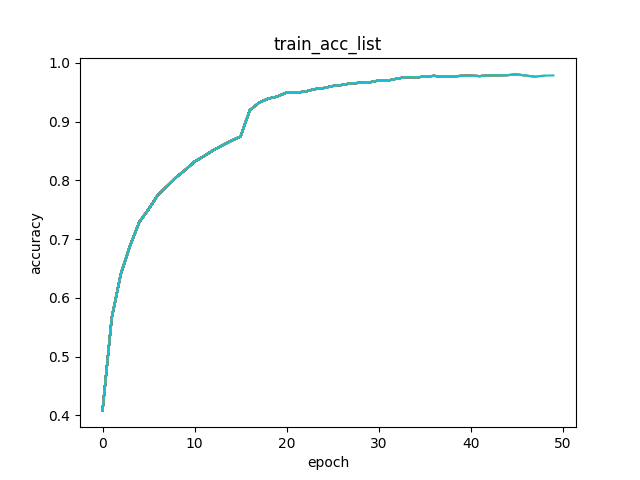
\includegraphics[scale=0.5]{p2/experiment/mynet_2024_04_14_21_58_22_sgd_pre_da/log/train_acc_list.png} & 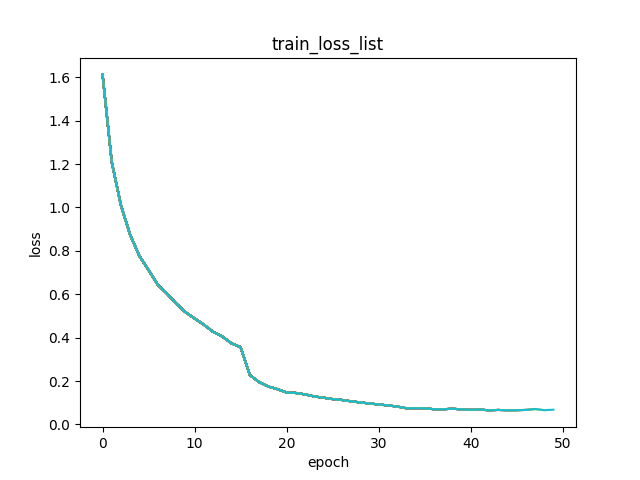
\includegraphics[scale=0.5]{p2/experiment/mynet_2024_04_14_21_58_22_sgd_pre_da/log/train_loss_list.png} \\
        \hline
        valid &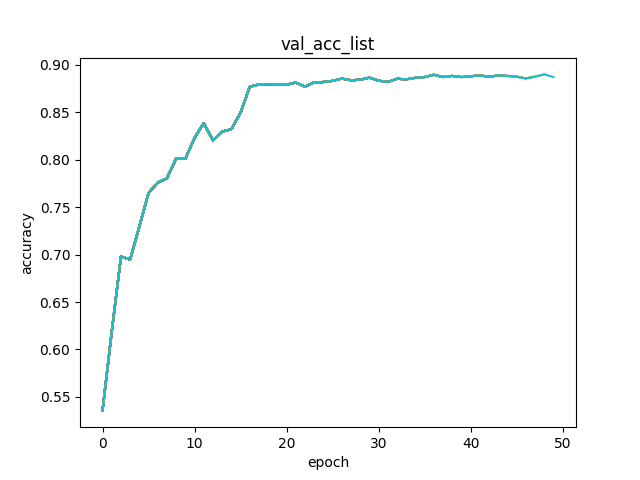
\includegraphics[scale=0.5]{p2/experiment/mynet_2024_04_14_21_58_22_sgd_pre_da/log/val_acc_list.png} & 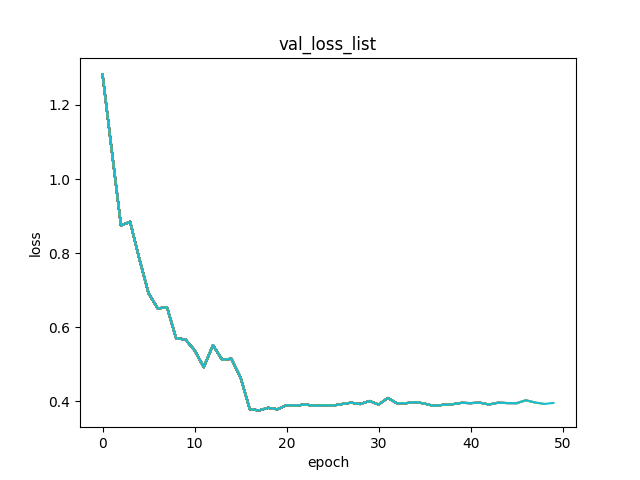
\includegraphics[scale=0.5]{p2/experiment/mynet_2024_04_14_21_58_22_sgd_pre_da/log/val_loss_list.png} \\
        \hline
    \end{tabular}
\end{table}

\begin{table}[!htb]
    \centering
    \caption{The learning curves of the training process (train/validation) for resnet18 models}
    \begin{tabular}{|c|c|c|}
        \hline
        type & accuracy & loss \\
        \hline
        train &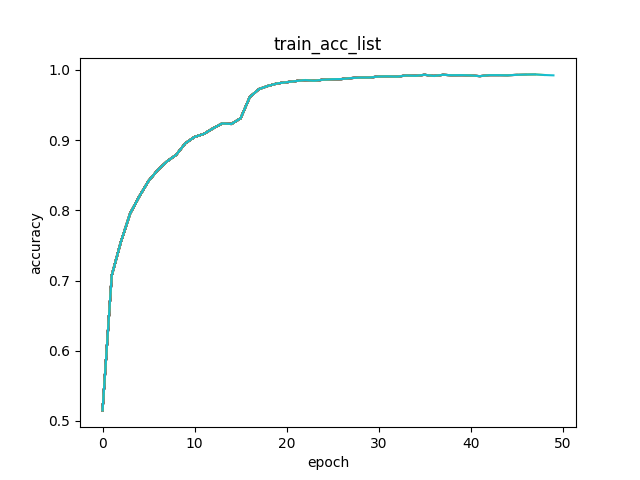
\includegraphics[scale=0.5]{p2/experiment/resnet18_2024_04_12_14_05_14_sgd_pre_da/log/train_acc_list.png} & 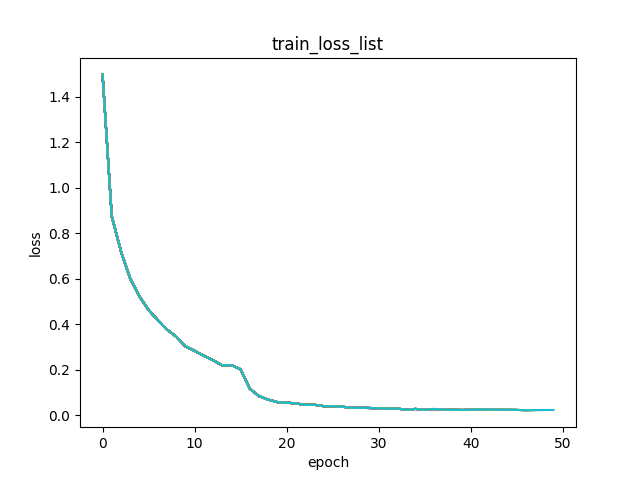
\includegraphics[scale=0.5]{p2/experiment/resnet18_2024_04_12_14_05_14_sgd_pre_da/log/train_loss_list.png} \\
        \hline
        valid &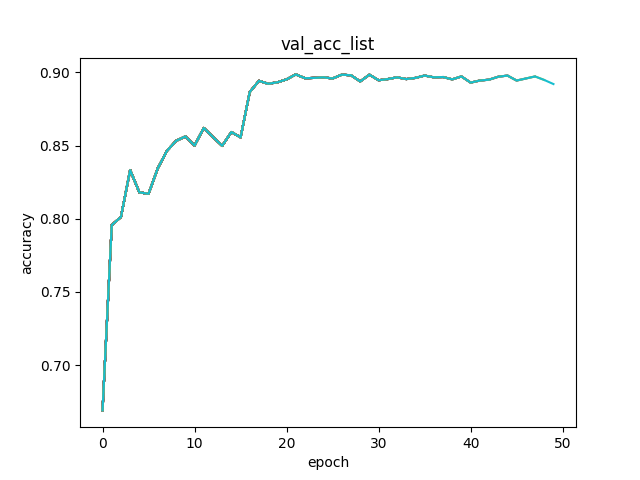
\includegraphics[scale=0.5]{p2/experiment/resnet18_2024_04_12_14_05_14_sgd_pre_da/log/val_acc_list.png} & 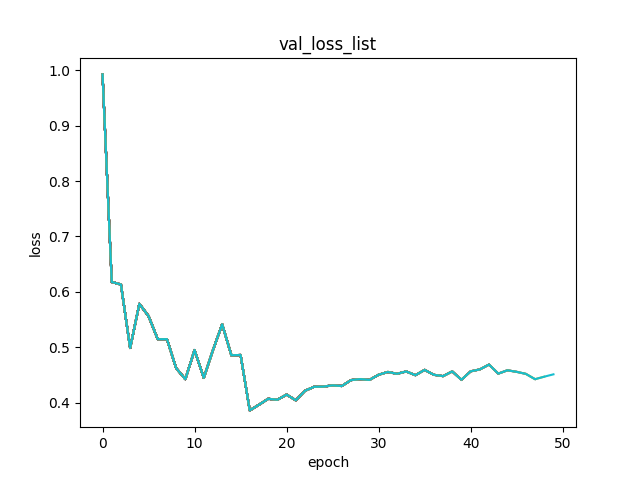
\includegraphics[scale=0.5]{p2/experiment/resnet18_2024_04_12_14_05_14_sgd_pre_da/log/val_loss_list.png} \\
        \hline
    \end{tabular}
\end{table}

\vspace{10em}

\subsection{Briefly describe what method do you apply on your best model? (e.g. data augmentation, model architecture, loss function, etc) (10\%)}
To ensure the stability of the program, I initially focused on developing and optimizing a ResNet18 model.  Considering the rotational invariance challenge of CNNs,  I introduced random rotation into the data augmentation process. Following recommendations from the task guidelines, I optimized the model by reducing the kernel size and stride of the first convolution layer, while also eliminating the first max-pooling layer and replacing it with Identity(). Surprisingly, these adjustments resulted in the model passing the strong baseline (0.84) in its first training iteration.

In pursuit of comparable accuracy and performance to the resnet18, I evaluated the VGG16\cite{simonyan2015deep} and VGG19\cite{simonyan2015deep} CNN models, given their similar release times compared to resnet18. Notably, I observed that VGG19 exhibited lower accuracy compared to VGG16 during the training process. To address the failure to pass the strong baseline,  I attempted to optimize the VGG16 model by introducing the dropout strategy and increasing the dimensions of the first two convolutional layers from $64$ to $96$, this led to an increment of accuracy from 0.825 to 0.8316. 

Despite several modifications, optimizing the model architecture alone did not yield the desired accuracy enhancements. Hence, I incorporated data augmentation techniques into the training process again and found that applying random horizontal flip techniques to images consistently improved model accuracy. With this addition, the model surpassed the strong baseline (0.84). However, I noticed that the model size exceeds the 80MB size limitation, so I began exploring all other known CNN models to address this constraint.

\vspace{2em}

The CNN models that I experimented with included LeNet\cite{726791}, AlexNet\cite{NIPS2012_c399862d}, GoogleNet\cite{szegedy2014going}, and DenseNet\cite{huang2018densely}. The results revealed that LeNet and AlexNet had relatively low accuracies and failed to meet the strong baseline (0.84). Only GoogleNet and DenseNet surpassed the strong baseline (0.84), achieving accuracies of 0.8898 and 0.876, respectively. Consequently, I opted for GoogleNet as the final model choice.

To improve the GoogleNet model, I attempted to fine-tune its architecture. Firstly, I consolidated the preceding convolution layers into a single convolution layer.  Inspired by the advancements in architectures like Inception V2, V3, and V4, one extra layer is added to the convolution block of branch 3. Additionally, I referenced PyTorch to adjust the kernel size from 5 to 3 on branch 3. Finally, I introduced dropout to mitigate superfluous information, ultimately producing my customized version of the GoogleNet model.

% BibTex
\bibliographystyle{ieeetr}
\bibliography{reference}

\end{document}